\section{Sensorknoten}
Die Entwicklerdokumentation für die \skk fasst alle relevanten Informationen zusammen, die für eine Weiterentwicklung der \skfw und des Installationstools benötigt werden.
Diese umfassen die verwendeten Repositorien, Steps to Code, die Code"=Konventionen, die Projektstruktur, die Steps to Debug und die Code"=Dokumentation.

\subsection{Repositorien}
In diesem Abschnitt werden die Repositorien für die \skfw und das Installationstool beschrieben.
\Tbl{skfwrepos}  listet diese auf.

\begin{table}[htb]
	\caption{Repositorien der \skk und ihr Zweck}
	\begin{tabular}{|p{45mm}|p{93mm}|}
		\hline
		Name & Zweck \\ \hline
		Firmware"=sensornode & \skfw die im Rahmen des \schit entwickelt wurde (veraltet) \\ \hline
		sensornode"=firmware & Aktuelle \skfw \\ \hline
		sensornode"=schit"=migration & \skfw zur Migration von der \schit"=\skfw auf die aktuelle \skfw \\ \hline
		rioinstaller & Installationstool auf Basis von QT5 (C++), das im Rahmen des \schit entwickelt wurde (veraltet) \\ \hline
		sensornode"=config"=tool & Aktuelles Installationstool (C\#) \\ \hline
		sensornode"=bme280"=adapter & NodeMCU"= Firmware um einen BME280 über USB unter Ubuntu anzuschließen (debugging) \\ \hline
	\end{tabular}
	\label{tbl:skfwrepos}
\end{table}

Da der Großteil des Codes der \skk im \reponame{sensornode"=firmware}"=Repositorium erarbeitet wurde, beziehen sich folgende Abschnitte ausschließlich darauf.

\subsection{Projektstruktur}
In diesem Abschnitt werden die Ordnerstruktur, die Kompilate der \skk und deren externe Abhängigkeiten behandelt.

\subsubsection{Ordnerstruktur}
\label{sec:skFolderStructure}
Folgende Ordnerstruktur ist vorgesehen:

\begin{itemize}
	\item \textbf{root}:             Git-, Docker-, Jenkinsdateien, make.sh, etc.
	\item \textbf{config}:           Ein vollständiges Beispiel für die Konfigurations"=Datei des Sensorknotens + Unit"=Test Config"=Dateien
	\item \textbf{fs\_data}:         Alle Dateien, die auf das Filesystem des ESP8266 aufgespielt werden
	\item \textbf{include}:          Plattformspezifische .h-Dateien
	\item \textbf{lib}:              Gemeinsame Dateien für alle Plattformen (.h- und .cpp-Dateien)
	\item \textbf{makefiles}:        Die plattformspezifischen Make"=Dateien
	\item \textbf{readme\_assets}:   Assets für diese Dokumentation
	\item \textbf{src}:              Plattformspezifische .cpp-Dateien und die main.cpp
	\item \textbf{submodules}:       Die verwendeten Abhängigkeiten zu anderen Projekten (als git"=submodules)
	\item \textbf{test}:             Die Unit"=Tests
\end{itemize}

Die Ordner \dirname{include}, \dirname{src}, \dirname{lib} und \dirname{test} enthalten Unterordner, die im Wesentlichen der Architektur der \skfw entsprechen.

\subsubsection{Kompilate und Externe Abhängigkeiten}
Der Source"=Code der \skfw kann für verschiedene Zwecke und Zielsysteme kompiliert werden.
In \Tbl{sktargetsystems} sind diese aufgelistet.

\begin{table}[htb]
	\caption{Zwecke und Zielsysteme der \skfw}
	\begin{tabular}{|p{0.2\linewidth}|p{0.15\linewidth}|p{0.55\linewidth}|}
		\hline
		Zweck & Zielsystem & Erläuterung \\ \hline
		\skfw & NodeMCU & Firmware zum Aufspielen auf die Node"-MCU \\ \hline
		Debugging & Native (x86) & Portierung der Firmware für Linux"=Basierte Systeme zum Debuggen \\ \hline
		Test & Native (x86) & Wird für die Testausführung verwendet (basierend auf Native) \\ \hline
	\end{tabular}
	\label{tbl:sktargetsystems}
\end{table}

Da für die verschiedenen Zielsysteme der \skfw ebenfalls unterschiedliche Bibliotheken und Frameworks verwendet werden, sind diese zur Übersicht in \Tbl{skextfw} aufgelistet.
Die Einbindung derer wird in \Tbl{sklinking} erläutert.

\begin{table}[htb]
	\caption{Externe Abhängigkeiten der \skfw}
	\begin{tabular}{|p{0.23\linewidth}|p{0.22\linewidth}|p{0.16\linewidth}|p{0.27\linewidth}|}
		\hline
		Name & Version & Verwendung & Einbindung \\ \hline
		esp8266 & 2.5.0 & NodeMCU & Entwickler"=Rechner \\ \hline
		Esp""Software""Serial & 3.4.2 & NodeMCU & Entwickler"=Rechner \\ \hline
		make""Esp""Arduino & 4.18.0 & NodeMCU & Git"=Submodule \\ \hline
		SparkFun BME""280 Arduino Library & 2.0.4 & NodeMCU & modifizierte Kopie \\ \hline
		pubsubclient & v2.7 & NodeMCU & Git"=Submodule \\ \hline
		libserial & latest (25.03.""'19) & Native & Entwickler"=Rechner \\ \hline
		paho.mqtt.c & latest (15.04.""'19) & Native & Entwickler"=Rechner \\ \hline
		paho.mqtt.cpp & latest (06.05.""'19) & Native & Entwickler"=Rechner \\ \hline
		ArduinoJSON & 6.x & Alle & Git"=Submodule \\ \hline
		googletest & release"=1.8.1 & Test & Git"=Submodule \\ \hline
		Fakeit & 2.0.5 & Test & Git"=Submodule \\ \hline
	\end{tabular}
	\label{tbl:skextfw}
\end{table}

\begin{table}[htb]
	\caption{Einbindung der externen Abhängigkeiten der \skfw}
	\begin{tabular}{|p{0.20\linewidth}|p{0.74\linewidth}|}
		\hline
		Einbindung & Erläuterung \\ \hline
		Entwickler"=Rechner & Muss auf dem Entwickler"=Rechner installiert sein, um das Projekt kompilieren zu können. Wird durch das Installations"=Script in \Fref{sec:sk:stepsToCode} abgedeckt. \\ \hline
		Git"=Submodule & Ist als Git"=Submodule im Projekt eingebunden. \\ \hline
		modifizierte Kopie & Code"=Dateien aus der Abhängigkeit sind in dieses Projekt kopiert und angepasst. Sie liegen neben den Eigenimplementierungen. \\ \hline
	\end{tabular}
	\label{tbl:sklinking}
\end{table}

Eine vollständige Tabelle samt Lizenzen, Links und Erläuterung ist in \Tbl{skextfwfull} abgebildet.
Weitere Erläuterungen zu den Lizenzen sind in \Tbl{sklicenses} beschrieben.

\subsection{Steps to Code}
\label{sec:sk:stepsToCode}
In diesem Abschnitt wird die Vorgehensweise beschrieben, mit der ein (neuer) Entwickler zum Projekt beitragen kann.
Im Folgenden werden die erforderlichen Schritte aufgelistet:

\begin{enumerate}
	\item{Ein Debian basiertes System (VM) mit bash, apt, firefox und sudo Rechte für den aktuellen Benutzer aufsetzen.}
	\item{Zugriff auf das \reponame{sensornode"=firmware}"=Repositorium erlangen.}
	\item{Die Datei \filename{setup\_vm.sh} in das oben genannte System herunterladen, ein Terminal im selben Ordner öffnen und das Skript mit \console{bash setup\_vm.sh} ausführen.}
	\begin{itemize}
		\item{Alternativ mit \console{chmod +x setup\_vm.sh \&\& ./setup\_vm.sh}.}
	\end{itemize}
	\item{Auf Nachfrage die benötigten Daten eingeben, die Nachfrage zu einer unbeobachteten Installation (unattended mode) bejahen und einen Kaffee (oder ein anderes Getränk) trinken gehen, während das Skript alles vorbereitet.}
	\item{Im Terminal mit \console{cd \textasciitilde/sensornode-firmware} in die lokale Kopie des Repositorium wechseln.}
	\item{Mit \console{code .} \textit{Visual Studio Code} starten und anfangen zu Programmieren.}
	\item{Optional:}
	\begin{enumerate}
		\item{Mit \console{./make.sh all} die Firmware für alle Plattformen (Native und Node"=MCU) bauen.}
		\item{Den Sensorknoten nach Standard"=Schaltplan (siehe \Fig{skwiringdefault}) zusammen bauen.}
		\item{Mit \console{./make.sh nodemcu\_v2\_fs\_upload} das Dateisystem aufspielen.}
		\item{Mit \console{./make.sh nodemcu\_v2\_upload} die Firmware aufspielen.}
	\end{enumerate}
\end{enumerate}

\begin{figure}[htb]
	\centering
	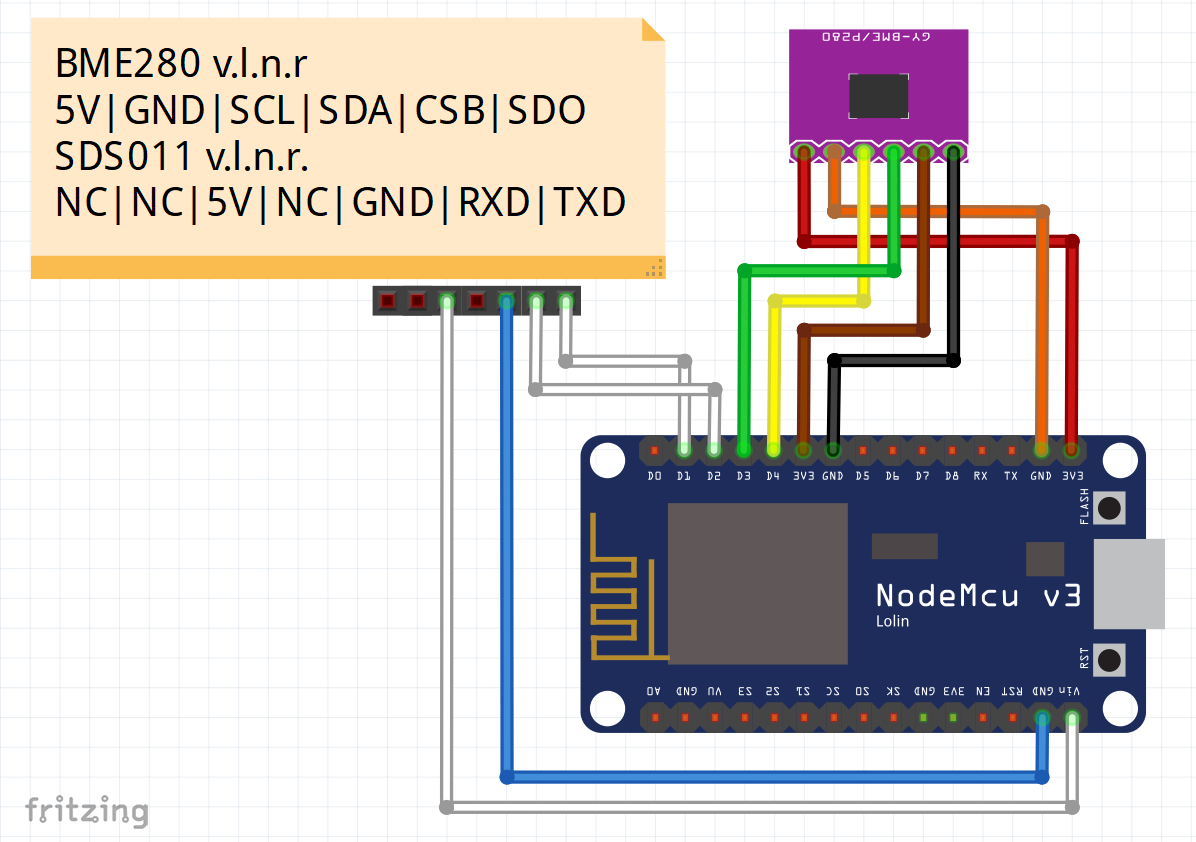
\includegraphics[width=0.7\linewidth]{./ressourcen/Prod_Verdrahtungsplan}
	\caption{Der Standard"=Verdrahtungsplan für den \sk}
	\label{fig:skwiringdefault}
\end{figure}

\subsection{Unit"=Tests}
Da in der \pg als Vorgehensmodell TDD festgelegt wurde, existieren für die \skfw Unit"=Tests.
Diese sind in der Ordnerstruktur unter \dirname{test} zu finden (siehe \Fref{sec:skFolderStructure}).
Die Testausführung geschieht ebenfalls über das \console{make.sh}"=Skript.
Dabei ist zu beachten, dass die Dateien \filename{config.json}, \filename{credentials.json} und die \filename{mergedConfig.json} im Ordner \dirname{config} vorhanden sind.
Die \filename{mergedConfig.json} ist dabei die zusammengefügte \filename{.json}"=Datei aus \filename{config.json} und \filename{credentials.json}.
Konfigurationsänderungen, beschrieben im Dokument III, Abschnitt 1.4.4, müssen somit ebenfalls in der \filename{mergedConfig.json} vorgenommen werden, da sonst die Unit"=Tests fehlschlagen.
Die Ausführung der Unit"=Tests geschieht dann im Repositorium der \skfw mit \console{./make.sh test}.
Zu empfehlen ist hierbei auch das vorhergehende Aufräumen der alten Build"=Artefakte mittels \console{./make.sh clean}.

\subsection{Code"=Aufbau}
Der Code"=Aufbau folgt im Wesentlichen der Architektur in \Fref{sec:skArchitektur}, jedoch sind einige Komponenten nicht in der Architektur enthalten, da sie gesondert zu behandeln sind.
Diese werden in diesem Abschnitt erläutert.

\subsubsection{Bootstrapper}
Der \code{Bootstrapper} ist dazu da, die Konfiguration aus der \filename{config.json} und \filename{credentials.json} zu verarbeiten und die benötigten Objekte daraus zu erstellen.
Jede Komponente aus der Architektur wird hier initialisiert.
Außerdem erzeugt der \code{Bootstrapper} den \code{Scheduler} zum Verwalten der Tasks und die \code{Sensornode} als übergeordnetes Objekt, das den \code{Scheduler} beinhaltet.
Plattformspezifische Initialisierungen werden durch Vererbung an den \code{NodeMcuBootstrapper} und \code{NativeBootstrapper} delegiert.

\subsubsection{SensorNode}
Die \code{SensorNode} war ursprünglich als Container für alle dynamischen Objekte gedacht.
Durch die Verwendung von \textit{Smart"=Pointern} und einer frühen Umstrukturierung der Code"=Basis dient die \code{SensorNode} nun nur noch dazu, den \code{Scheduler} aufzurufen.

\subsubsection{Scheduler}
Der \code{Scheduler} dient dazu, alle Tasks im \textit{Round"=Robin"=Verfahren} aufzurufen.
Dabei ruft er die \code{act()}"=Methode des aktiven Tasks solange auf, bis entweder der Zeitschlitz von \SI{25}{ms} verstrichen ist, oder der Task kein \code{ITask::State} \code{::busy} als Rückgabewert liefert.
Zusätzlich bricht der Scheduler die Ausführung der Tasks ab, sobald ein Task \code{ITask::State::error} als Rückgabewert liefert.
Dies hat einen Programmabbruch, oder im Falle der NodeMCU einen Neustart, zur Folge.

\subsubsection{Platform}
Das \code{Platform}"=Objekt dient als Abstraktionsschicht zu stellenweise benötigten plattformspezifischen Funktionen.
Diese werden durch Vererbung bereitgestellt.
Folgende Aufzählung listet Funktionalitäten auf:
\begin{itemize}
	\item \code{FileWrapper}: Operationen auf dem Dateisystem ausführen.
	\item \code{NodeMcuPlatformFactory}: Erzeugt den \code{FileWrapper}.
	\item \code{SerialWrapper}: Operationen auf der seriellen Schnittstelle ausführen.
	\item \code{NodeMcuServerConnectionFactory}: Erzeugt TCP"=Verbindungen (nicht in Native implementiert).
	\item \code{NodeMcuSystemStatusWrapper}: Liefert Statusinformationen zum System (nicht in Native implementiert).
\end{itemize}

\subsubsection{StringPool}
Das \code{StringPool}"=Objekt ist als Container für alle im Code verwendeten Strings vorgesehen.
Die Idee dahinter ist, dass alle Strings an einer Stelle gesammelt werden, um unnötige Duplikate im Speicher zu vermeiden.
Die Strings können im Code über \textit{enum}"=Werte und entsprechenden \code{get}"=Funktionen referenziert werden.
Als geplante, aber noch nicht implementierte, Funktionalität sollten die Strings entweder in den Programmspeicher, oder sogar in das Dateisystem, ausgelagert werden, um Speicherplatz im RAM zu sparen.
Durch die bislang geringe Anzahl an Strings wurde dies allerdings nicht umgesetzt.

\subsection{Firmware"=Updates}
In diesem Abschnitt werden die Firmware"=Updates behandelt.
Firmware"=Updates werden in der Develop-Umgebung per HTTP über den Server \url{https://pg-rio-strg.informatik.uni-oldenburg.de} bezogen.
Dieser muss dazu im Webroot eine JSON"=Datei mit dem Namen \filename{availableUpdates.json} und folgendem Aufbau bereitstellen:
\begin{lstlisting}[language=json]
{
  "updates": [
    {
      "_v": "1",
      "path": "/realtivePathTo.bin",
      "version": "version",
      "crc32": "crc32inLowerLetters",
      "description": "Description"
    },
    {
      "_v": "1",
      "path": "/files/empty.bin",
      "version": "0.0.190911000000",
      "crc32": "deadbeef",
      "description": "Example-File"
    }
  ]
}
\end{lstlisting}

Die Firmware"=Datei wird dann relativ zur \filename{availableUpdates.json} abgelegt, hier im Beispiel im Verzeichnis \dirname{files}.
Da der Puffer für die \filename{availableUpdates.json}"=Datei auf dem Sensorknoten begrenzt ist, sollten nicht mehr als fünf Versionen in der Datei zur Verfügung stehen.
Die Auswertung der \filename{availableUpdates.json} geschieht dann "von oben nach unten", wobei die erste Firmware mit neuerer Version ausgewählt und heruntergeladen wird.
Dieses Vorgehen ermöglicht eine gezielte Sequenzialisierung der Updates, sofern einmal eine Interims"=Firmware benötigt werden sollte. 


\subsection{Code"=Konventionen}
In diesem Abschnitt werden die Code"=Konventionen beschrieben, die in dem \reponame{sensornode"=firmware}"=Repositorium verwendet werden.
In den anderen Repositorien aus \tbl{skfwrepos} gelten keine Code"=Konventionen.

\subsubsection{Code"=Styling}
Für das Styling des Codes wird das Tool clang"=format verwendet.
Die Definition der Formatierung ist in der Datei \filename{.clang"=format} im Wurzelverzeichnis des Projekts zu finden.
Die Korrektheit des Stylings wird durch den Jenkins"=Job überprüft und kann durch die Verwendung von \console{./make.sh format} oder die Verwendung von Extensions in VS Code (Clang"=Format ermöglicht die Formatierung beim Speichern einer Datei) angewandt werden.

\subsubsection{Namenskonventionen}
In diesem Projekt werden durchweg \textit{telling names} verwendet.
Das heißt die Namen von Variablen, Funktionen und Klassen sollten ihre Funktionalität möglichst genau beschreiben.
Dabei sollen die Namen aber so kurz wie möglich, aber so lang wie nötig gehalten werden.
Darüberhinaus gibt es folgende Konventionen zur Benennung innerhalb dieses Projekts:

\begin{itemize}
	\item Sind in Klassen, die nicht von \code{ITask} ableiten, Arbeitsaufrufe notwendig, so sind diese Funktionen mit \code{act()} zu benennen. (Im Gegensatz zum \code{call()} in \code{ITask})
	\item Werden \code{unique\_ptr<T>} durch Funktionen an einen neuen Owner übergeben, so ist die Funktion mit \code{take\textit{Something}()} zu benennen.
	\item Erfolgt eine Kommunikation mit einer Klasse, die als State Machine implementiert ist, welche den internen Zustand der State Machine ändert, so ist die Funktion mit \code{trigger\textit{Something}()} zu benennen.
\end{itemize}

\subsubsection{C/C++"=Konventionen}
Folgende C/C++"=Konventionen sollten befolgt werden:

\begin{itemize}
	\item In \code{for}"=Schleifen wird der Inkrement"=Operator \code{++i} (nicht \code{i++}) verwendet.
	\item Es werden durchweg smart pointers (gegenüber raw pointers) verwendet. Siehe Guidelines.
	\item Es werden \textit{enum classes} verwendet, siehe z.B. \code{DataSinkNames} im Projekt.
	\item Bei überschriebenen Methoden ist \code{override} bzw. \code{final} zu ergänzen.
	\item State Machines werden mit \code{std::function} implementiert. Dies ist vor allem beim Refactoring vorhandener State"=Machines im \code{switch/case}"=Style zu beachten.
\end{itemize}

Ausnahmen von diesen Regeln, sind mittels Code"=Kommentar zu begründen.
Des Weiteren wurden die Regeln im Laufe der \pg erweitert, sodass sie nicht durchgehend Anwendung fanden.

\subsubsection{C++"=Guidelines}
\begin{itemize}
	\item \url{http://isocpp.github.io/CppCoreGuidelines/CppCoreGuidelines}
	\item \url{https://www.heise.de/developer/artikel/C-Core-Guidelines-Interfaces-I-3767608.html}
	\item \url{https://www.heise.de/developer/artikel/C-Core-Guidelines-Regeln-fuer-Smart-Pointer-3919901.html}
\end{itemize}

\subsection{Steps to Debug}
Für das Debugging gibt es zwei vorgesehene Möglichkeiten.
Die erste ist das Ausführen der Sensorknoten"=Software auf dem Entwicklerrechner.
Dabei können die Debug"=Funktionalitäten von Visual Studio Code verwendet werden.
Der Nachteil dieser Variante ist, dass nicht die Produktivsoftware vollumfänglich getestet werden kann.
Also können nicht alle Fehler aufgedeckt werden (insbesondere Fehler im plattformspezifischen Code).
Bei der zweiten Variante werden Debug"=Ausgaben in den Code eingebunden, um das Verhalten des Programms auf dem Sensorknoten zu analysieren.
Die Debug"=Firmware kann dann mit \console{./make.sh nodemcu\_v2\_debug} \console{ \&\& ./make.sh nodemcu\_v2\_debug\_upload} erzeugt und auf den Sensorknoten eingespielt und gestartet werden.
Zudem muss der PIN D4 der NodeMCU an einen USB"=Serial"=Converter angeschlossen werden (siehe \Fig{skwiringdebug}), um die Debug"=Ausgaben (115200 Baud, 8N1) am Rechner anzeigen zu können.
Diese Variante ist aufwändiger, aber kann auch Fehler im NodeMCU"=spezifischen Code aufdecken.

\begin{figure}[htb]
	\centering
	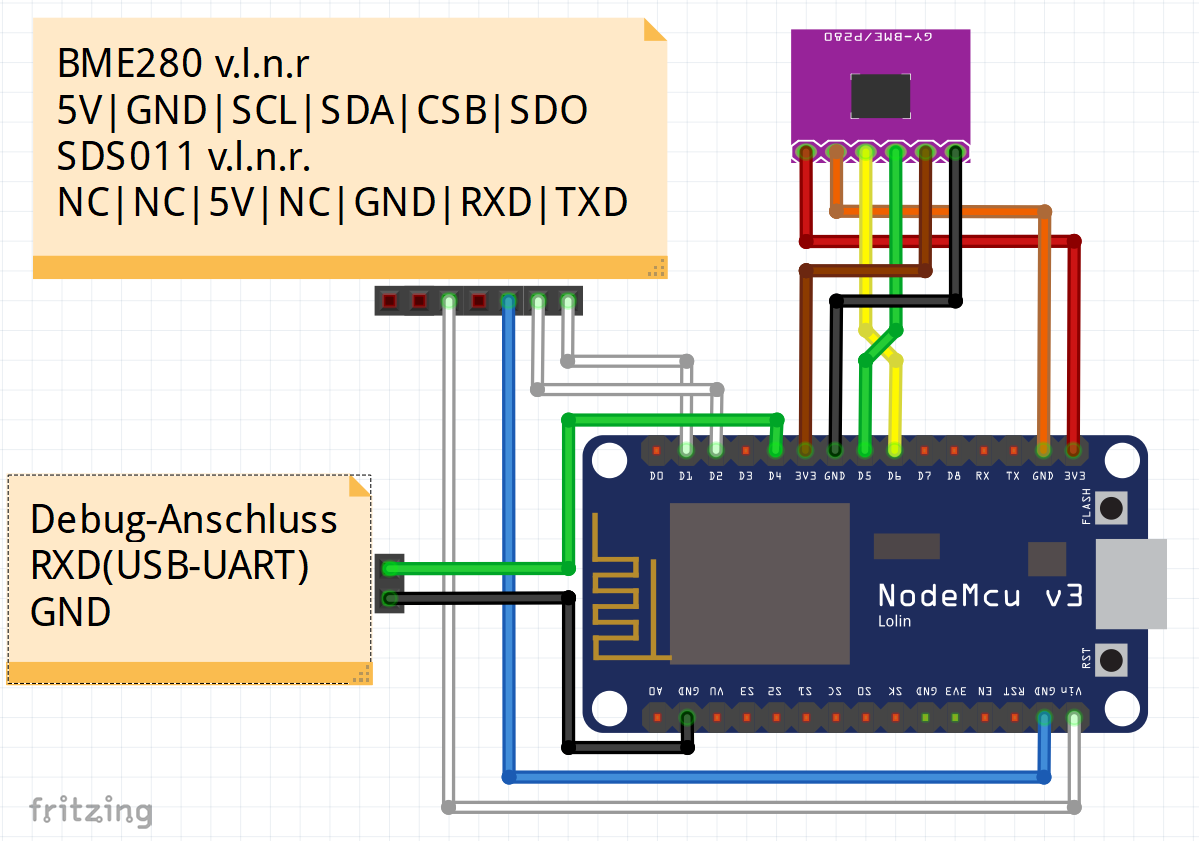
\includegraphics[width=0.7\linewidth]{./ressourcen/Prod_Verdrahtungsplan_Debug}
	\caption{Der Debug"=Verdrahtungsplan für den \sk}
	\label{fig:skwiringdebug}
\end{figure}

\subsection{Dokumentation}
In diesem Abschnitt werden die Dokumentationsrichtlinien für die \skk behandelt.
Diese teilen sich in die Code"=Dokumentation und Architektur auf.

\subsubsection{Code"=Dokumentation}
Die Codedokumentation der Interfaces und Klassen erfolgt in den zugehörigen h"=Dateien.
Es muss mindestens eine Beschreibung zum Interface bzw. der Klasse angegeben und darüber hinaus alle öffentlichen Funktionen und Enums dokumentiert werden.
Konstruktoren und Destruktoren werden nur im Ausnahmefall erläutert.
Aus den Codekommentaren wird mittels Doxygen automatisch eine Dokumentation im HTML"=Format generiert.
Dazu wird der Befehl \console{./make.sh code\_docu} verwendet.
Zudem wird die Dokumentation bei der Ausführung des Jenkins"=Jobs erstellt und als Artefakt in einer ZIP"=Datei archiviert.

\subsubsection{Architektur}
\label{sec:skArchitektur}
Die Dokumentation der Architektur der \skfw wird im Repositorium \reponame{dokumentation}\footnote{\url{https://git.swl.informatik.uni-oldenburg.de/projects/PGRIO/repos/dokumentation/browse}} vorgenommen.
Dort sind zum einen die Beschreibung der Architektur, die sich als Fließtext in den Gesamttext einfügt, und zum anderen im Unterverzeichnis \dirname{ressourcen} die UML"=Modelle zu finden.

Bei Änderungen an der Architektur wird die Dokumentation immer zusammen mit der Implementierung (innerhalb des selben JIRA"=Tickets) gepflegt.

\subsection{Konfigurationstool}
Das PGRIO"=SK"=Config"=Tool ist ein Windows"=Programm zur Installation und Konfiguration der Firmware für den Sensorknoten der Projektgruppe RiO.
Mit dem Tool kann die aktuelle Firmware aus dem Internet heruntergeladen und auf dem ESP8266 geflasht werden.
Zusätzlich können Konfigurationsänderungen auf dem Sensorknoten vorgenommen werden.

\subsubsection{Technologie}
Dieses Projekt wird mit C\# und dem .NET"=Framework 4.7.2 mit Hilfe von WPF entwickelt.

\subsubsection{Entwicklungsumgebung}
Als Entwicklungsumgebung kommt die Community"=Edition von MS Visual Studio zum Einsatz.

\subsubsection{Deployment}
Es ist kein CI/CD"=Job für dieses Projekt angelegt.
Daher muss ein Deployment manuell durchgeführt werden.
Dazu wird das Projekt mit Visual Studio gebaut und die PGRIO"=SK"=Config"=Tool.exe am gewünschten Pfad veröffentlicht.
Die Produktiv"=Version wird auf der Website \url{https://pg-rio-uis.informatik.uni-oldenburg.de/mitmachen} als Download bereitgestellt.
Die exe"=Datei ist eigenständig (ohne zugehörige dll"=Dateien) ausführbar.

\subsubsection{Abhängigkeiten}
Es gibt die in \Tbl{skctdependencies} dargestellten Abhängigkeiten im Projekt.

\begin{table}[htb]
	\caption{Externe Abhängigkeiten des Konfigurationstools}
	\begin{tabular}{|p{0.14\linewidth}|p{0.20\linewidth}|p{0.07\linewidth}|p{0.08\linewidth}|p{0.14\linewidth}|p{0.20\linewidth}|}
		\hline
		Name & Verweis & Lizenz & Version & Einbindung & Erläuterung \\ \hline
		Caliburn. Micro & \url{https://caliburnmicro.com} & MIT & 3.2.0 & nuget"=Paket & Framework für DataBindings mit MVVM"=Pattern in WPF \\ \hline
		Crc32.NET & \url{https://github.com/force-net/Crc32.NET} & MIT & 1.2.0 & nuget"=Paket & Framework zur Berechnung einer CRC32"=Prüfsumme \\ \hline
		esptool"=ck & \url{https://github.com/igrr/esptool-ck} & GPL-2.0 & 0.4.13 & .exe als Embedded"=Resource & Tool zum Flashen der Firmware auf den ESP8266 \\ \hline
		NewtonSoft. Json & \url{https://www.newtonsoft.com/json} & MIT & 12.0.2 & nuget"=Paket & Framework zum Verarbeiten von JSON \\ \hline
	\end{tabular}
	\label{tbl:skctdependencies}
\end{table}
